\chapter{Modelowanie systemu i jego otoczenia}
\label{cha:modelowanie_systemu}

W~niniejszym rozdziale opracowano modele analityczno-projektowe w~języku UML, przedstawiające funkcjonalności, procesy, interakcje oraz zachowania projektowanego systemu.


% ==============================================================================
\section{Diagram przypadków użycia}
\label{sec:diagram_przypadkow_uzycia}

W~niniejszym podrozdziale przedstawiono model funkcjonalny systemu w~postaci diagramu przypadków użycia UML, obejmujący identyfikację aktorów, wykaz zdefiniowanych przypadków użycia, ich powiązanie z~wymaganiami funkcjonalnymi oraz specyfikacje przebiegu wybranych procesów.


\subsection{Identyfikacja aktorów}
\label{subsec:identyfikacja_aktorow}

W~ramach projektowanego systemu zdefiniowano dwóch kluczowych aktorów wchodzących w~interakcję z~aplikacją:

\begin{itemize}
    \item \textbf{Użytkownik} -- główny aktor pierwszoplanowy (kierowca lub właściciel pojazdu), który wprowadza dane o~tankowaniach i~kosztach, analizuje statystyki zużycia paliwa/energii, zarządza profilami aut oraz konfiguruje przypomnienia.
    \item \textbf{System Android} -- aktor pomocniczy (systemowy), reprezentujący środowisko wykonawcze urządzenia mobilnego. Odpowiada za realizację zaplanowanych zadań w~tle i~wyzwalanie lokalnych powiadomień w~wyznaczonych terminach.
\end{itemize}

\clearpage

\subsection{Zestawienie przypadków użycia}
\label{subsec:zestawienie_przypadkow_uzycia}

W~wyniku analizy celów aktorów oraz zakresu funkcjonalnego wyodrębniono przypadki użycia projektowanego systemu, które zestawiono w~tabeli~\ref{tab:zestawienie_przypadkow_uzycia}.

\begin{table}[H]
    \centering
    \caption{Zestawienie przypadków użycia systemu}
    \label{tab:zestawienie_przypadkow_uzycia}
    \renewcommand{\arraystretch}{1.3}
    \begin{tabularx}{\linewidth}{|>{\centering\arraybackslash}p{2.2cm}|X|>{\centering\arraybackslash}p{5.5cm}|}
        \hline
        \rowcolor{tableheader}
        \textbf{Identyfikator} & \multicolumn{1}{c|}{\textbf{Nazwa przypadku użycia}} & \textbf{Aktor} \\
        \hline
        \hypertarget{uc:UC01}{UC01} & Zarządzanie profilami pojazdów & Użytkownik \\
        \hline
        \hypertarget{uc:UC02}{UC02} & Przełączanie aktywnego pojazdu & Użytkownik \\
        \hline
        \hypertarget{uc:UC03}{UC03} & Rejestracja wpisu tankowania & Użytkownik \\
        \hline
        \hypertarget{uc:UC04}{UC04} & Obliczenie średniego zużycia paliwa/energii & Wykorzystywany przez UC03 \\
        \hline
        \hypertarget{uc:UC05}{UC05} & Kalkulacja zasięgu i~symulacja kosztów & Użytkownik \\
        \hline
        \hypertarget{uc:UC06}{UC06} & Rejestracja wydatku eksploatacyjnego & Użytkownik \\
        \hline
        \hypertarget{uc:UC07}{UC07} & Konfiguracja i~edycja przypomnień & Rozszerzający UC06 \\
        \hline
        \hypertarget{uc:UC08}{UC08} & Wyzwalanie lokalnego powiadomienia & System Android \\
        \hline
        \hypertarget{uc:UC09}{UC09} & Generowanie analiz i~prognozy budżetowej & Użytkownik \\
        \hline
        \hypertarget{uc:UC10}{UC10} & Przeglądanie i~edycja historii eksploatacji & Użytkownik \\
        \hline
        \hypertarget{uc:UC11}{UC11} & Rozpoznawanie danych z~paragonu (OCR) & Rozszerzający UC03 \\
        \hline
    \end{tabularx}
    \zrodlo{Opracowanie własne.}
\end{table}

\clearpage

\subsection{Diagram przypadków użycia}
\label{subsec:diagram_uc}

Na rysunku~\ref{fig:diagram_przypadkow_uzycia} przedstawiono diagram przypadków użycia projektowanego systemu.

\begin{figure}[H]
    \centering
    % diagram przypadków użycia z Software Ideas Modeler 
    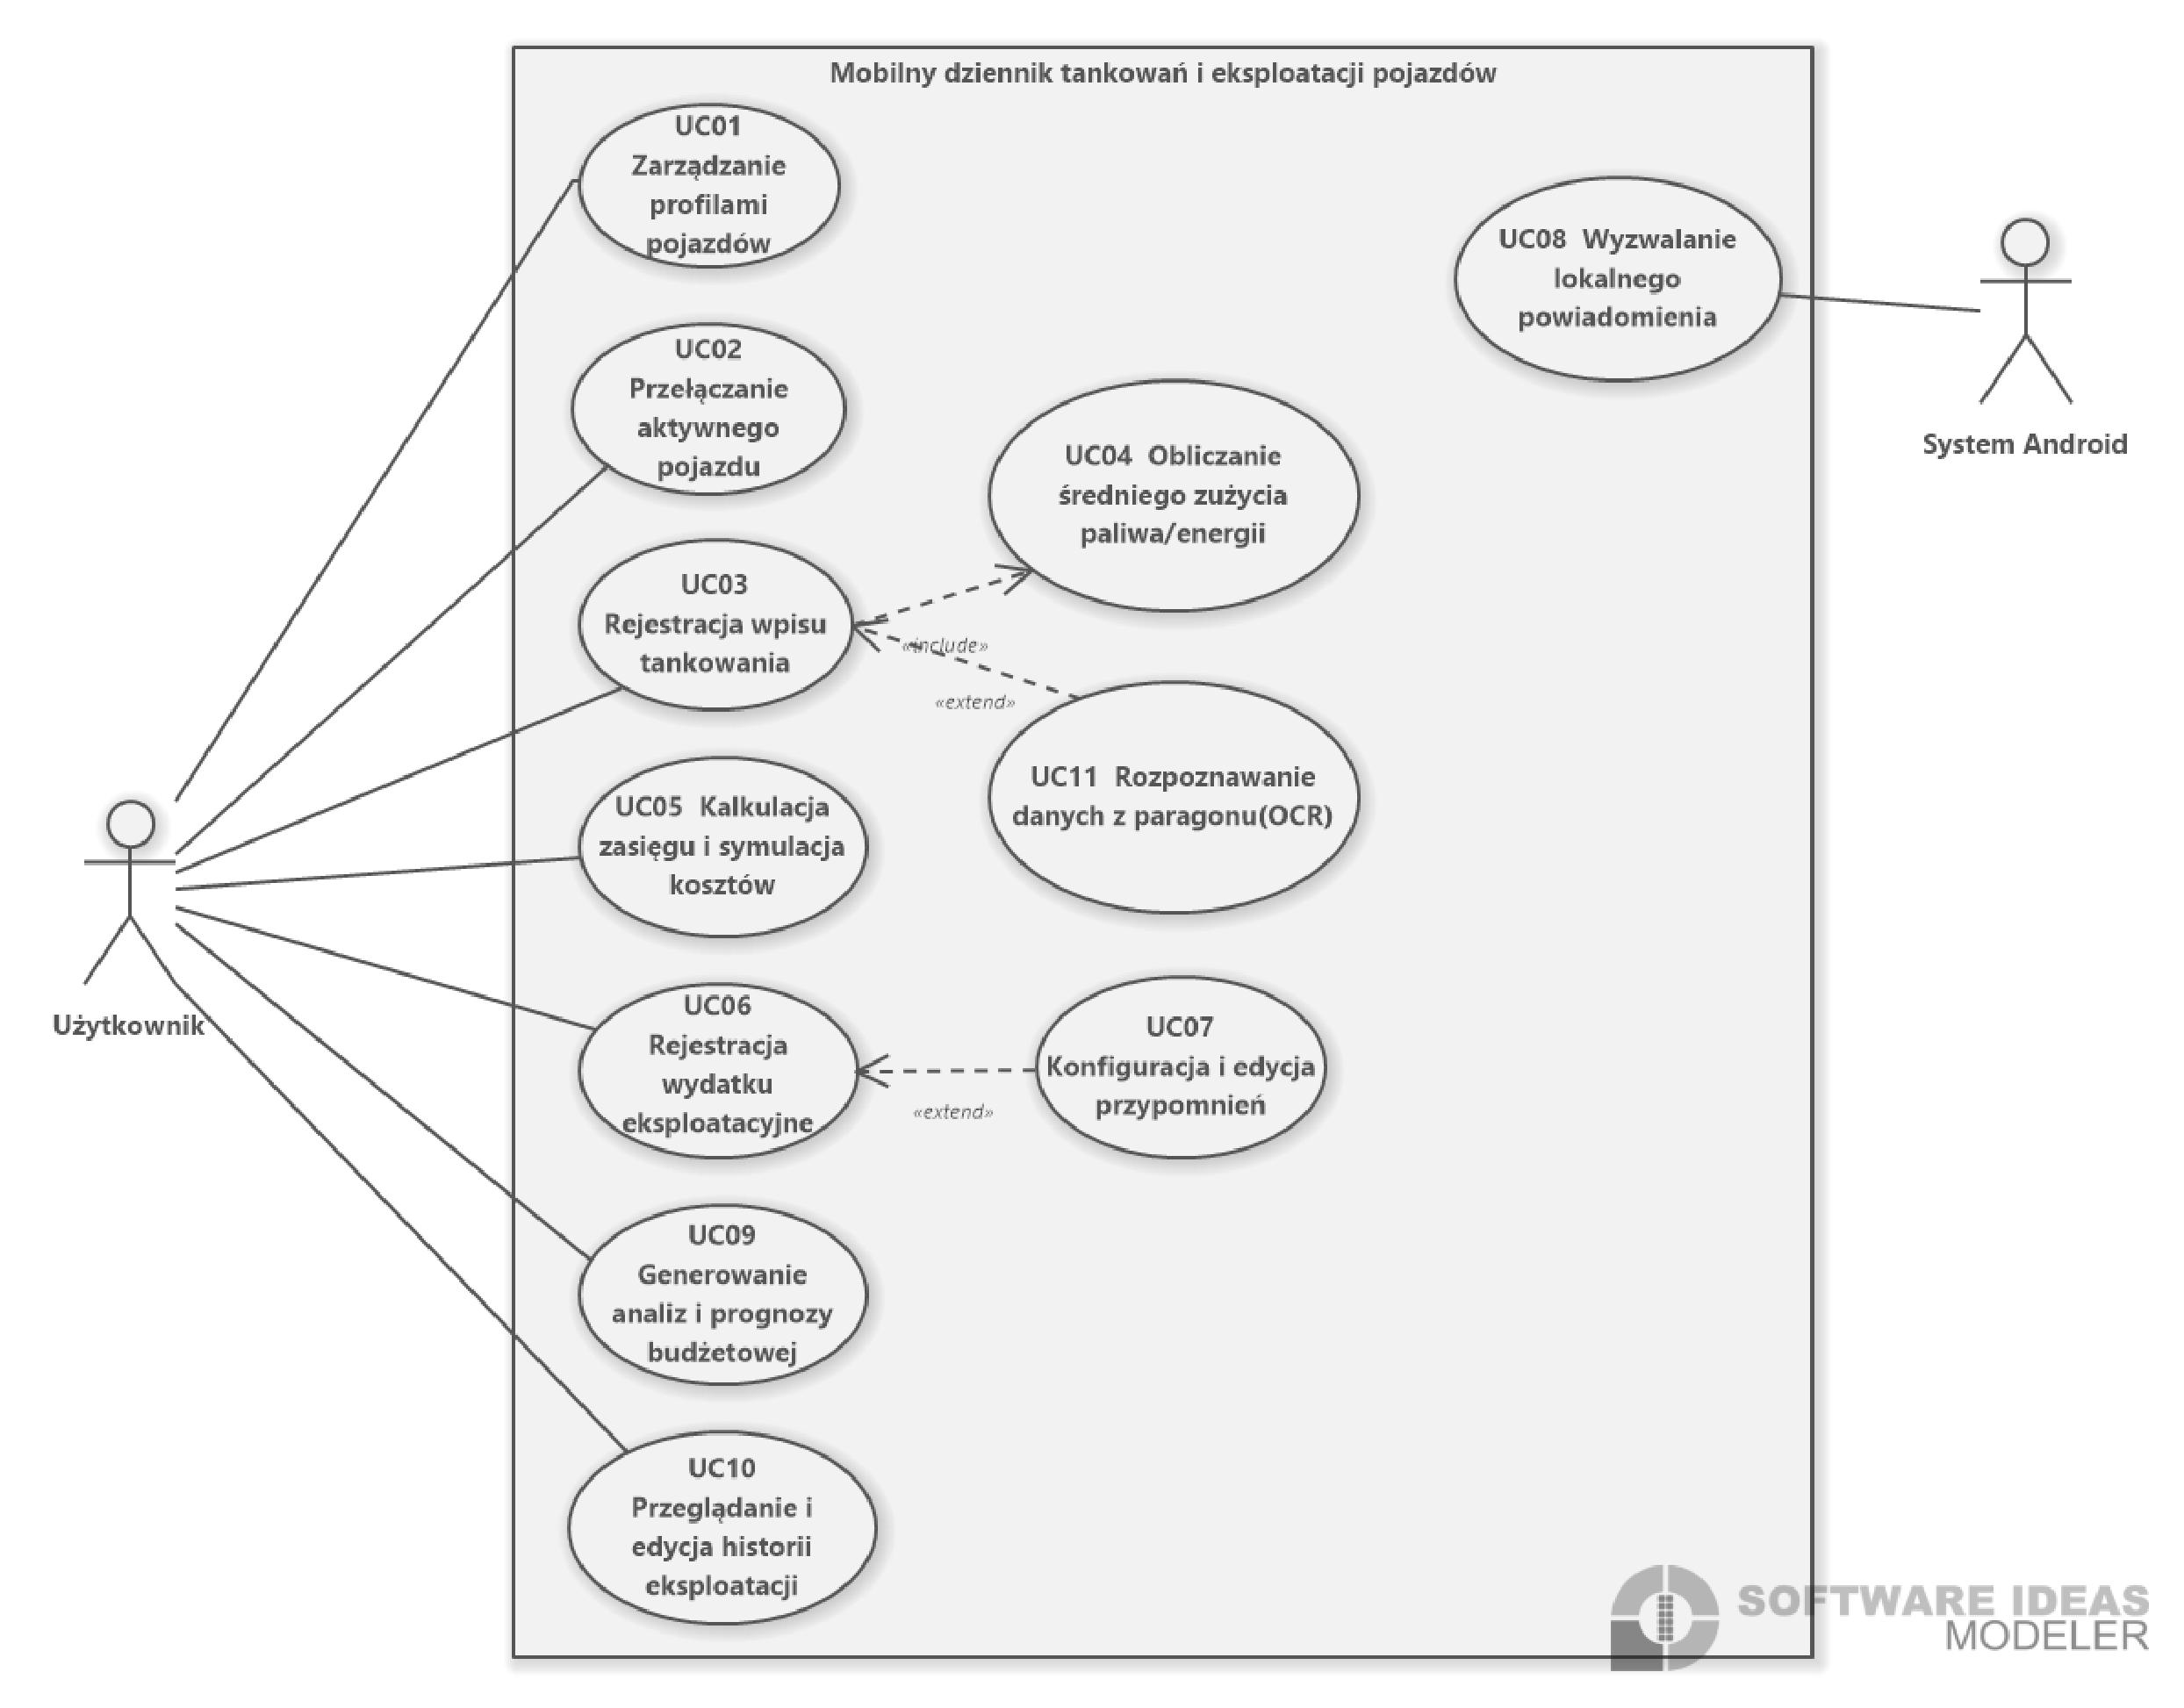
\includegraphics[width=0.98\linewidth]{figures/UseCaseDiagram1.eps}
    \caption{Diagram przypadków użycia}
    \label{fig:diagram_przypadkow_uzycia}
    \zrodlo{Opracowanie własne przy użyciu Software Ideas Modeler.}
\end{figure}

Na diagramie zastosowano relację «include» między przypadkami UC03 i~UC04 -- wyliczenie średniego zużycia paliwa/energii jest obowiązkowym elementem zapisu pełnego tankowania. Relację «extend» wykorzystano przy przypadkach UC11 (opcjonalne pobranie danych z~paragonu przez moduł OCR) oraz UC07 (opcjonalne zdefiniowanie przypomnienia podczas rejestracji wydatku). Pozostałe linie na diagramie stanowią asocjacje wskazujące udział aktorów w~realizacji poszczególnych operacji.

\clearpage

\subsection{Powiązanie wymagań funkcjonalnych z diagramem}
\label{subsec:powiazanie_wf_diagram}

Każde wymaganie funkcjonalne zdefiniowane w~rozdziale~\ref{cha:analiza_wymagan} znajduje odzwierciedlenie w~modelu przypadków użycia. Zestawienie powiązań przedstawiono w~tabeli~\ref{tab:powiazanie_wf_diagram}.

\begin{table}[H]
    \centering
    \caption{Powiązanie wymagań funkcjonalnych z~diagramem przypadków użycia}
    \label{tab:powiazanie_wf_diagram}
    \renewcommand{\arraystretch}{1.3}
    \begin{tabularx}{\linewidth}{|>{\centering\arraybackslash}p{1.5cm}|X|>{\centering\arraybackslash}p{2.6cm}|>{\centering\arraybackslash}p{2.2cm}|}
        \hline
        \rowcolor{tableheader}
        \textbf{ID} & \multicolumn{1}{c|}{\textbf{Wymaganie funkcjonalne}} & \textbf{Aktor} & \textbf{Przypadek użycia} \\
        \hline
        \hyperlink{wf:WF-01}{WF-01} & Dodawanie i~edycja profili pojazdów ze zdjęciem. & Użytkownik & \hyperlink{uc:UC01}{UC01} \\
        \hline
        \hyperlink{wf:WF-02}{WF-02} & Rejestracja tankowania z~automatycznym przeliczaniem kwot. & Użytkownik & \hyperlink{uc:UC03}{UC03} \\
        \hline
        \hyperlink{wf:WF-03}{WF-03} & Automatyczne obliczanie średniego zużycia paliwa/energii. & ------ & \hyperlink{uc:UC04}{UC04} \\
        \hline
        \hyperlink{wf:WF-04}{WF-04} & Wyliczanie przewidywanego zasięgu pojazdu. & Użytkownik & \hyperlink{uc:UC05}{UC05} \\
        \hline
        \hyperlink{wf:WF-05}{WF-05} & Rejestracja wydatków eksploatacyjnych z~kategoriami. & Użytkownik & \hyperlink{uc:UC06}{UC06} \\
        \hline
        \hyperlink{wf:WF-06}{WF-06} & Planowanie przypomnień i~wyzwalanie powiadomień w~tle. & Użytkownik / System Android & \hyperlink{uc:UC07}{UC07}, \hyperlink{uc:UC08}{UC08} \\
        \hline
        \hyperlink{wf:WF-07}{WF-07} & Generowanie miesięcznej prognozy wydatków. & Użytkownik & \hyperlink{uc:UC09}{UC09} \\
        \hline
        \hyperlink{wf:WF-08}{WF-08} & Przełączanie aktywnego widoku między pojazdami. & Użytkownik & \hyperlink{uc:UC02}{UC02} \\
        \hline
        \hyperlink{wf:WF-09}{WF-09} & Przeglądanie i~edycja historii eksploatacji. & Użytkownik & \hyperlink{uc:UC10}{UC10} \\
        \hline
        \hyperlink{wf:WF-10}{WF-10} & Zapis i~odczyt danych w~lokalnej bazie offline. & ------ & \hyperlink{uc:UC01}{UC01}, \hyperlink{uc:UC03}{UC03}, \hyperlink{uc:UC06}{UC06}, \hyperlink{uc:UC10}{UC10} \\
        \hline
        \hyperlink{wf:WF-11}{WF-11} & Skanowanie paragonu i~odczyt danych przez moduł OCR. & Użytkownik & \hyperlink{uc:UC11}{UC11} \\
        \hline
    \end{tabularx}
    \zrodlo{Opracowanie własne na podstawie analizy wymagań.}
\end{table}


\clearpage

\subsection{Szczegółowe specyfikacje przypadków użycia}
\label{subsec:scenariusze_przypadkow_uzycia}

W~niniejszej sekcji przedstawiono szczegółowe specyfikacje tabelaryczne dla dwóch wybranych przypadków użycia: przypadku UC03 (wykorzystującego relację «include») oraz przypadku UC06 (wykorzystującego relację «extend»).


\subsubsection{Specyfikacja przypadku użycia UC03: Rejestracja wpisu tankowania}
\label{subsubsec:specyfikacja_uc1}

Podstawowe parametry przypadku użycia UC03 zestawiono w~tabeli~\ref{tab:specyfikacja_uc1_parametry}.

\begin{table}[H]
    \centering
    \caption{Parametry przypadku użycia UC03}
    \label{tab:specyfikacja_uc1_parametry}
    \renewcommand{\arraystretch}{1.3}
    \begin{tabularx}{\linewidth}{|>{\bfseries\arraybackslash}p{4.2cm}|X|}
        \hline
        \rowcolor{tableheader}
        \multicolumn{1}{|c|}{\textbf{Element}} & \multicolumn{1}{c|}{\textbf{Opis}} \\
        \hline
        Identyfikator & UC03 \\
        \hline
        Nazwa & Rejestracja wpisu tankowania \\
        \hline
        Aktor główny & Użytkownik \\
        \hline
        Cel & Wprowadzenie danych o~zrealizowanym tankowaniu, aktualizacja stanu licznika pojazdu oraz obliczenie średniego zużycia paliwa/energii. \\
        \hline
        Warunki początkowe & Aplikacja jest uruchomiona, a~w~systemie istnieje co najmniej jeden aktywny profil pojazdu. \\
        \hline
        Powiązania & «include» UC04~--~Obliczenie średniego zużycia paliwa/energii, «extend» UC11~--~Rozpoznawanie danych z~paragonu (OCR) \\
        \hline
        Warunki końcowe -- sukces & Nowy wpis tankowania został zapisany w~bazie danych, stan licznika pojazdu zaktualizowany, a~w~przypadku tankowania do pełna wyliczono średnie spalanie. \\
        \hline
        Warunki końcowe -- niepowodzenie & Wpis nie został zapisany. System wyświetlił komunikat o~błędzie walidacji i~pozostawił formularz do poprawy. \\
        \hline
    \end{tabularx}
    \zrodlo{Opracowanie własne.}
\end{table}

\clearpage

Przebieg główny przypadku użycia przedstawiono w~tabeli~\ref{tab:przebieg_glowny_uc1}.

\begin{table}[H]
    \centering
    \caption{Przebieg główny przypadku użycia UC03}
    \label{tab:przebieg_glowny_uc1}
    \renewcommand{\arraystretch}{1.3}
    \begin{tabularx}{\linewidth}{|>{\centering\arraybackslash}p{1.2cm}|X|X|}
        \hline
        \rowcolor{tableheader}
        \textbf{Krok} & \multicolumn{1}{c|}{\textbf{Działanie aktora}} & \multicolumn{1}{c|}{\textbf{Odpowiedź systemu}} \\
        \hline
        1 & Wybiera opcję dodania nowego tankowania. & Wyświetla formularz z~podpowiedzią bieżącej daty i~ostatniego stanu licznika. \\
        \hline
        2 & Wprowadza stan licznika, ilość paliwa oraz łączny koszt (ręcznie lub skanując paragon przez \hyperlink{uc:UC11}{UC11}). & Na bieżąco przelicza cenę za litr przy zmianie kwoty (\hyperlink{rb:RB-04}{RB-04}). \\
        \hline
        3 & Zatwierdza formularz przyciskiem zapisu. & Sprawdza poprawność przebiegu (\hyperlink{rb:RB-01}{RB-01}) oraz daty (\hyperlink{rb:RB-05}{RB-05}) i~wylicza średnie spalanie (\hyperlink{uc:UC04}{UC04}, \hyperlink{rb:RB-02}{RB-02}). \\
        \hline
        4 & --- & Zapisuje wpis w~bazie danych (\hyperlink{wf:WF-10}{WF-10}) i~aktualizuje stan licznika pojazdu. \\
        \hline
        5 & --- & Wyświetla potwierdzenie zapisu, prezentuje wyliczone spalanie i~odświeża ekran główny. \\
        \hline
    \end{tabularx}
    \zrodlo{Opracowanie własne.}
\end{table}

\clearpage

Warianty alternatywne oraz obsługę wyjątków przedstawiono w~tabeli~\ref{tab:scenariusz_alt_uc1}.

\begin{table}[H]
    \centering
    \caption{Scenariusze alternatywne i~wyjątkowe dla przypadku użycia UC03}
    \label{tab:scenariusz_alt_uc1}
    \renewcommand{\arraystretch}{1.3}
    \begin{tabularx}{\linewidth}{|>{\centering\arraybackslash}p{1.4cm}|X|X|}
        \hline
        \rowcolor{tableheader}
        \textbf{Krok} & \multicolumn{1}{c|}{\textbf{Działanie aktora}} & \multicolumn{1}{c|}{\textbf{Odpowiedź systemu}} \\
        \hline
        \multicolumn{3}{|l|}{\cellcolor{tableheader!50}\textbf{Wariant A1 -- Stan licznika mniejszy od poprzedniego (\hyperlink{rb:RB-01}{RB-01})}} \\
        \hline
        A1.1 & --- & Wykrywa, że wprowadzony stan licznika jest mniejszy lub równy wartości z~poprzedniego wpisu. \\
        \hline
        A1.2 & --- & Blokuje zapis, podświetla pole przebiegu i~wyświetla komunikat błędu. \\
        \hline
        A1.3 & Poprawia wartość przebiegu. & Weryfikuje nową wartość i~usuwa komunikat błędu. \\
        \hline
        A1.4 & Ponownie zatwierdza formularz. & Powraca do weryfikacji w~kroku~3 przebiegu głównego. \\
        \hline
        \multicolumn{3}{|l|}{\cellcolor{tableheader!50}\textbf{Wariant A2 -- Rejestracja z~datą wsteczną (\hyperlink{rb:RB-05}{RB-05})}} \\
        \hline
        A2.1 & --- & Wykrywa, że data wpisu jest wcześniejsza niż data poprzedniego tankowania. \\
        \hline
        A2.2 & --- & Wyświetla okno ostrzegawcze o~możliwym zaburzeniu statystyk z~opcją kontynuacji lub anulowania. \\
        \hline
        A2.3 & Wybiera anulowanie zapisu lub potwierdza kontynuację. & Po anulowaniu umożliwia poprawę daty; po potwierdzeniu przechodzi do zapisu w~kroku~4. \\
        \hline
        A2.4 & Wprowadza skorygowaną datę i~ponawia zapis. & Powraca do kroku~3 przebiegu głównego. \\
        \hline
        \multicolumn{3}{|l|}{\cellcolor{tableheader!50}\textbf{Wariant A3 -- Niepełny odczyt danych z~paragonu (\hyperlink{uc:UC11}{UC11})}} \\
        \hline
        A3.1 & --- & Moduł OCR nie jest w~stanie poprawnie odczytać wszystkich pól z~fotografii. \\
        \hline
        A3.2 & --- & Wyświetla informację o~częściowym odczycie i~uzupełnia tylko rozpoznane wartości. \\
        \hline
        A3.3 & Ręcznie uzupełnia brakujące dane w~formularzu. & Sprawdza poprawność wprowadzonych wartości. \\
        \hline
        A3.4 & Zatwierdza uzupełniony formularz przyciskiem zapisu. & Powraca do kroku~3 przebiegu głównego. \\
        \hline
    \end{tabularx}
    \zrodlo{Opracowanie własne.}
\end{table}


\clearpage

\subsubsection{Specyfikacja przypadku użycia UC06: Rejestracja wydatku eksploatacyjnego}
\label{subsubsec:specyfikacja_uc2}

Podstawowe parametry przypadku użycia UC06 zestawiono w~tabeli~\ref{tab:specyfikacja_uc2_parametry}.

\begin{table}[H]
    \centering
    \caption{Parametry przypadku użycia UC06}
    \label{tab:specyfikacja_uc2_parametry}
    \renewcommand{\arraystretch}{1.3}
    \begin{tabularx}{\linewidth}{|>{\bfseries\arraybackslash}p{4.2cm}|X|}
        \hline
        \rowcolor{tableheader}
        \multicolumn{1}{|c|}{\textbf{Element}} & \multicolumn{1}{c|}{\textbf{Opis}} \\
        \hline
        Identyfikator & UC06 \\
        \hline
        Nazwa & Rejestracja wydatku eksploatacyjnego \\
        \hline
        Aktor główny & Użytkownik \\
        \hline
        Cel & Ewidencja kosztu eksploatacyjnego (np. naprawa, ubezpieczenie, badanie techniczne) z~możliwością zaplanowania przypomnienia o~nadchodzącym terminie. \\
        \hline
        Warunki początkowe & Aplikacja jest uruchomiona, a~w~systemie istnieje co najmniej jeden aktywny profil pojazdu. \\
        \hline
        Powiązania & «extend» UC07~--~Konfiguracja i~edycja przypomnień \\
        \hline
        Warunki końcowe -- sukces & Informacja o~wydatku została zapisana w~bazie danych, a~zaplanowane powiadomienia zarejestrowano w~systemie. \\
        \hline
        Warunki końcowe -- niepowodzenie & Wydatek nie został zapisany. System wyświetlił komunikat o~brakujących lub błędnych danych formularza. \\
        \hline
    \end{tabularx}
    \zrodlo{Opracowanie własne.}
\end{table}

Przebieg główny przypadku użycia przedstawiono w~tabeli~\ref{tab:przebieg_glowny_uc2}.

\begin{table}[H]
    \centering
    \caption{Przebieg główny przypadku użycia UC06}
    \label{tab:przebieg_glowny_uc2}
    \renewcommand{\arraystretch}{1.3}
    \begin{tabularx}{\linewidth}{|>{\centering\arraybackslash}p{1.2cm}|X|X|}
        \hline
        \rowcolor{tableheader}
        \textbf{Krok} & \multicolumn{1}{c|}{\textbf{Działanie aktora}} & \multicolumn{1}{c|}{\textbf{Odpowiedź systemu}} \\
        \hline
        1 & Przechodzi do modułu kosztów i~wybiera dodanie nowego wydatku. & Wyświetla formularz z~wyborem kategorii, kwotą, datą oraz opcją przypomnień. \\
        \hline
        2 & Wybiera kategorię okresową (np. ubezpieczenie), podaje kwotę i~datę. & Weryfikuje dane i~proponuje automatyczne przypomnienie 7~dni przed terminem (\hyperlink{rb:RB-03}{RB-03}). \\
        \hline
        3 & Przechodzi do konfiguracji przypomnień (\hyperlink{uc:UC07}{UC07}). & Umożliwia modyfikację terminu powiadomienia oraz dodanie kolejnych terminów. \\
        \hline
        4 & Zatwierdza formularz przyciskiem zapisu. & Zapisuje wydatek w~bazie danych (\hyperlink{wf:WF-10}{WF-10}) oraz rejestruje zaplanowane powiadomienia. \\
        \hline
        5 & --- & Wyświetla potwierdzenie zapisu i~odświeża listę wydatków. \\
        \hline
    \end{tabularx}
    \zrodlo{Opracowanie własne.}
\end{table}

\clearpage

Scenariusz alternatywny A1 dla przypadku UC06 przedstawiono w~tabeli~\ref{tab:scenariusz_alt_uc2}.

\begin{table}[H]
    \centering
    \caption{Scenariusz alternatywny A1 dla przypadku użycia UC06}
    \label{tab:scenariusz_alt_uc2}
    \renewcommand{\arraystretch}{1.3}
    \begin{tabularx}{\linewidth}{|>{\centering\arraybackslash}p{1.4cm}|X|X|}
        \hline
        \rowcolor{tableheader}
        \textbf{Krok} & \multicolumn{1}{c|}{\textbf{Działanie aktora}} & \multicolumn{1}{c|}{\textbf{Odpowiedź systemu}} \\
        \hline
        A1.1 & Pozostawia opcję przypomnień wyłączoną (np. wydatek jednorazowy). & Pomija konfigurację powiadomienia (\hyperlink{uc:UC07}{UC07}) i~oczekuje na zatwierdzenie. \\
        \hline
        A1.2 & Zatwierdza formularz przyciskiem zapisu. & Zapisuje wydatek w~bazie danych (\hyperlink{wf:WF-10}{WF-10}) bez planowania powiadomień. \\
        \hline
        A1.3 & --- & Wyświetla potwierdzenie zapisu i~odświeża listę wydatków. \\
        \hline
    \end{tabularx}
    \zrodlo{Opracowanie własne.}
\end{table}


\clearpage

% ==============================================================================
\section{Diagramy aktywności}
\label{sec:diagramy_aktywnosci}



% Diagramy aktywności (\emph{Activity Diagrams}) przedstawiają przepływ sterowania, logikę biznesową oraz sekwencję czynności wykonywanych w~ramach modelowanych procesów z~uwzględnieniem węzłów decyzyjnych oraz rozgałęzień współbieżnych.


% \subsection{Diagram aktywności 1: [Nazwa pierwszego procesu, np. Proces rejestracji tankowania i obliczania spalania]}
% \label{subsec:diagram_aktywnosci_1}

% % TODO: Wprowadzenie do modelowanego procesu, opis jego znaczenia w systemie.

% \begin{figure}[H]
%     \centering
%     % Miejsce na diagram aktywności 1
%     % \includegraphics[width=0.8\linewidth]{figures/fig_act_tankowanie.pdf}
%     \caption{Diagram aktywności procesu [Nazwa procesu 1]}
%     \label{fig:diagram_aktywnosci_1}
%     \zrodlo{Opracowanie własne.}
% \end{figure}




% TODO: Szczegółowy opis diagramu aktywności 1:
% - kolejność wykonywanych czynności od stanu początkowego,
% - warunki decyzyjne (np. walidacja poprawności przebiegu, sprawdzenie flagi "do pełna"),
% - alternatywne ścieżki i obsługa wyjątków,
% - osiągnięcie stanu końcowego.




% \subsection{Diagram aktywności 2: [Nazwa drugiego procesu, np. Proces harmonogramowania i wyzwalania powiadomień serwisowych]}
% \label{subsec:diagram_aktywnosci_2}

% % TODO: Wprowadzenie do drugiego modelowanego procesu.

% \begin{figure}[H]
%     \centering
%     % Miejsce na diagram aktywności 2
%     % \includegraphics[width=0.8\linewidth]{figures/fig_act_powiadomienia.pdf}
%     \caption{Diagram aktywności procesu [Nazwa procesu 2]}
%     \label{fig:diagram_aktywnosci_2}
%     \zrodlo{Opracowanie własne.}
% \end{figure}

% TODO: Szczegółowy opis diagramu aktywności 2:
% - sekwencja operacji (tworzenie wpisu z datą przypomnienia, rejestracja zadania w WorkManager),
% - warunki weryfikacji terminu (np. reguła 7 dni przed terminem - RB-03),
% - ścieżki alternatywne (edycja terminu, anulowanie zadania, oznaczenie opłaty jako załatwiona),
% - wygenerowanie powiadomienia w systemie Android i stan końcowy.

% \clearpage

% ==============================================================================
\section{Diagramy sekwencji}
\label{sec:diagramy_sekwencji}

% Diagramy sekwencji (\emph{Sequence Diagrams}) obrazują dynamiczne zachowanie systemu oraz czasowy przebieg interakcji i~komunikacji pomiędzy uczestnikami (aktorami, widokami interfejsu, modelami widoku oraz warstwą bazy danych).


% \subsection{Diagram sekwencji 1: [Nazwa pierwszej interakcji, np. Dodanie tankowania i aktualizacja statystyk pojazdu]}
% \label{subsec:diagram_sekwencji_1}

% % TODO: Wprowadzenie do modelowanej sekwencji interakcji.

% \begin{figure}[H]
%     \centering
%     % Miejsce na diagram sekwencji 1
%     % \includegraphics[width=0.9\linewidth]{figures/fig_seq_tankowanie.pdf}
%     \caption{Diagram sekwencji interakcji [Nazwa interakcji 1]}
%     \label{fig:diagram_sekwencji_1}
%     \zrodlo{Opracowanie własne.}
% \end{figure}

% % TODO: Opis przebiegu analizowanego scenariusza:
% % - identyfikacja uczestników (np. :Użytkownik, :AddRefuelingScreen, :RefuelingViewModel, :RefuelingRepository, :RoomDatabase),
% % - zestawienie i kolejność przesyłanych komunikatów synchronicznych i asynchronicznych,
% % - zwracane odpowiedzi, walidacja i odświeżenie stanu interfejsu (StateFlow).


% \subsection{Diagram sekwencji 2: [Nazwa drugiej interakcji, np. Rejestracja wydatku eksploatacyjnego i harmonogramowanie powiadomienia]}
% \label{subsec:diagram_sekwencji_2}

% % TODO: Wprowadzenie do drugiej modelowanej interakcji.

% \begin{figure}[H]
%     \centering
%     % Miejsce na diagram sekwencji 2
%     % \includegraphics[width=0.9\linewidth]{figures/fig_seq_powiadomienia.pdf}
%     \caption{Diagram sekwencji interakcji [Nazwa interakcji 2]}
%     \label{fig:diagram_sekwencji_2}
%     \zrodlo{Opracowanie własne.}
% \end{figure}

% % TODO: Opis przebiegu analizowanego scenariusza:
% % - uczestnicy (np. :Użytkownik, :ExpenseScreen, :ExpenseViewModel, :ExpenseRepository, :WorkManager),
% % - sekwencja wywołań metod i planowania powiadomienia w tle,
% % - komunikaty zwrotne i obsługa błędów.


% \clearpage

% ==============================================================================
\section{Diagramy stanów}
\label{sec:diagramy_stanow}

% Diagramy maszyny stanów (\emph{State Machine Diagrams}) modelują cykl życia wybranych obiektów systemu, których zachowanie zmienia się w~odpowiedzi na zachodzące zdarzenia i~operacje.


% \subsection{Diagram stanów 1: [Nazwa pierwszego obiektu, np. Cykl życia profilu pojazdu]}
% \label{subsec:diagram_stanow_1}

% % TODO: Opis obiektu, dla którego modelowany jest stan (uzasadnienie biznesowe).

% \begin{figure}[H]
%     \centering
%     % Miejsce na diagram stanów 1
%     % \includegraphics[width=0.8\linewidth]{figures/fig_state_pojazd.pdf}
%     \caption{Diagram stanów obiektu [Nazwa obiektu 1]}
%     \label{fig:diagram_stanow_1}
%     \zrodlo{Opracowanie własne.}
% \end{figure}

% % TODO: Opis stanów, zdarzeń i przejść:
% % - możliwe stany (np. NowyNieaktywowany, AktywnyDomyślny, WycofanyZEksploatacji / Archiwalny),
% % - zdarzenia wyzwalające przejścia (np. wybór jako aktywny profil, edycja danych, archiwizacja),
% % - warunki dozorujące (strażnicy / guards) i akcje wejściowe/wyjściowe.


% \subsection{Diagram stanów 2: [Nazwa drugiego obiektu, np. Cykl życia zobowiązania eksploatacyjnego / przypomnienia]}
% \label{subsec:diagram_stanow_2}

% % TODO: Opis drugiego obiektu (np. Zobowiązanie / Przypomnienie o przeglądzie lub polisie OC).

% \begin{figure}[H]
%     \centering
%     % Miejsce na diagram stanów 2
%     % \includegraphics[width=0.8\linewidth]{figures/fig_state_przypomnienie.pdf}
%     \caption{Diagram stanów obiektu [Nazwa obiektu 2]}
%     \label{fig:diagram_stanow_2}
%     \zrodlo{Opracowanie własne.}
% \end{figure}

% % TODO: Opis stanów, zdarzeń i przejść:
% % - stany obiektu (np. Zaplanowane, Oczekujące, WymagająceUwagi / Powiadomione, Zrealizowane / Opłacone, Przeterminowane),
% % - zdarzenia (np. upływ czasu, nadejście bufora 7 dni - RB-03, potwierdzenie opłaty przez kierowcę, edycja terminu),
% % - podsumowanie cyklu życia obiektu.
